\documentclass[a4paper, 10pt]{article}
\title{MAT292---ODE}
\author{Jonah Chen}

\usepackage[utf8]{inputenc}
\usepackage[margin=0.5in]{geometry}

\usepackage{braket}
\usepackage{physoly}
\usepackage{currfile}
\usepackage{gensymb}
\usepackage{amssymb}
\usepackage{pgf,tikz,pgfplots}
\usepackage{mathrsfs}
\usepackage{textcomp}
\usetikzlibrary{arrows}
\numberwithin{equation}{section}
\pgfplotsset{compat=1.16}
\begin{document}

\maketitle
\tableofcontents

\section{Newton's Law of Cooling}
\begin{itemize}
    \item Newtons law of cooling states that
    \begin{equation}
        \frac{\dd u}{\dd t}=-k(u-T_0)
    \end{equation}
    \item Note that there is one trivial solution, the equilibrium solution is $u(t)=T_0$. The meaning of this solution is the temperature of an object doesn't change when it is already at the equilibrium temperature.
    \item \begin{align}
        \frac{\frac{\dd u}{\dd t}}{u-T_0}&=-k\\
        \frac{\dd}{\dd t}\log(u-T_0)&=-k\\
        \log(u-T_0)&=-kt+c_1\\
        u=T_0+\exp(c_1)\exp(-kt)&=T_0+c_2\exp(-kt)
    \end{align}
    Note that $c_2=\exp(c_1)>0$. However, this is not a complete solution as it cannot describe the solutions with $u<T_0$.
    \item \textbf{Warning:} note that the integral of $\frac{1}{x}$ is $\log|x|$, \textbf{NOT} $\log(x)$. This is what caused the solution to be incomplete.
    \item Hence, $c_2=\pm\exp(c_1)$. Note that $c_1=\pm\infty$ is allowed thus so $c_2$ can take any value.
    \item Below are the integral curves.
    % \begin{center}
    %     \begin{tikzpicture}
    %         \begin{axis}
    %             \addplot[domain=0:5]{60-15*exp(x)}
    %         \end{axis}
    %     \end{tikzpicture}
    % \end{center}
\end{itemize}

\section{Classifications}
\begin{definition}
    A differential equation is an equation containing one or more unknown functions of one or more independent variables.
\end{definition}

\begin{itemize}
    \item The order of a differential equation is the order of the highest derivative
    \item The most general n-th order ODE:
    \begin{equation}
        F[t,y,y',y'',\dots,y^{(n)}]=0
    \end{equation}
    \item Linear ODE.
    \item Autonomous ODE is an ODE which does not explicitly depend on the independent variable, like $y'=y$. $y'=ty$ is not autonomous.
    \item Seperable first order ODE is a first order ODE that can be written as $y'=p(t)q(y)$.
    \item Newton's Law of cooling is first order, linear, autonomous, and seperable. 
\end{itemize}

\section{Systems of Differential Equations}

\begin{itemize}
    \item Think of a zombie apocalypse. You need to find a good time to find food. 
    \item Let $x$ be the number of people, and $y$ be the number of zombles. This can be modelled by the \textit{Lotka--Volterra} or Predator--Prey equations.
    \begin{align}
        \derivative{x}{t}&=\alpha x-\beta xy\\
        \derivative{y}{t}&=-\gamma y+\delta xy
    \end{align}
    \item The term $\alpha x$ is inspired by short term population growth.
    \item The term $-\beta xy$ is inspired by the fact that zombies are eating people.
    \item The term $-\gamma y$ is inspired by the fact zombie die.
    \item The $\delta xy$ term is inspired by the fact that people can be converted to zombies.
    \item Note that this is \textbf{not} a linear equation. The term $xy$ is nonlinear. Let the dependent variable be $z=\begin{pmatrix}
        x\\y
    \end{pmatrix}$. Then $xy=z^T\begin{pmatrix}
        0&\frac{1}{2}\\\frac{1}{2}&0
    \end{pmatrix}$
    \item The most general quadratic form for vector (system of) equations is 
    \begin{align}
        z^TAz+b^Tz+c
    \end{align}
    \item Now take two twitter accounts, with each account telling its followers to unfollow the other account, with rates $m>0,n>0$ respectively. The accounts will naturally grow by word of mouth, with rates $k>0,l>0$ respectively. Note these constraints are important.
    \begin{align}
        p'&=kp-mo\\
        o'&=lo-np
    \end{align}
    \item There are oversimplification for this model. It ignores the fact that when somebody unfollows they cannot unfollow again.
\end{itemize}

\section{Qualitative Methods: Direction Fields and Phase Lines}
\begin{definition}
    Consider the ODE $y'=f(t,y)$. We can draw a \textbf{direction field} as follows:
    \begin{itemize}
        \item Draw a $t-y-$coordinate system.
        \item Evaluate $f(t,y)$ over a rectangular grid of points.
        \item Draw a line at each point $(t,y)$ of the grid with slope $f(t,y)$
    \end{itemize}
\end{definition}
\begin{itemize}
    \item Let's look again at Newton's law of cooling:
    \begin{equation}
        y'=-1.5(y-20)
    \end{equation}
    \begin{center}
        \includegraphics[width=0.7\textwidth]{mat292/fig1.png}
    \end{center}
    \item Based on the initial conditions, we can draw the approximate solution by following direction field.
    \item A lot of the behavior of the differential equation are visible from the slope field. 
\end{itemize}
\begin{definition}
    Consider an autonomous first-order ODE $y'=f(y)$.\\If $f(c)=0$ for a specific value $c$, we call $c$ an \textbf{equilibrium} of the ODE.\\We say it is
    \begin{enumerate}
        \item a \textbf{stable equilibrium}, if a solution starting at a value close to $c$ approaches $y=c$ as $t\to\infty$.
        \item an \textbf{unstable equilibrium}, if a solution starting at a value close to $c$ moves away from $y=c$ as $t\to\infty$.
        \item a \textbf{semistable equilibrium}, if we observe either behavior, depending on if the solution starts just above or below $c$.
    \end{enumerate}
\end{definition}
\begin{center}
    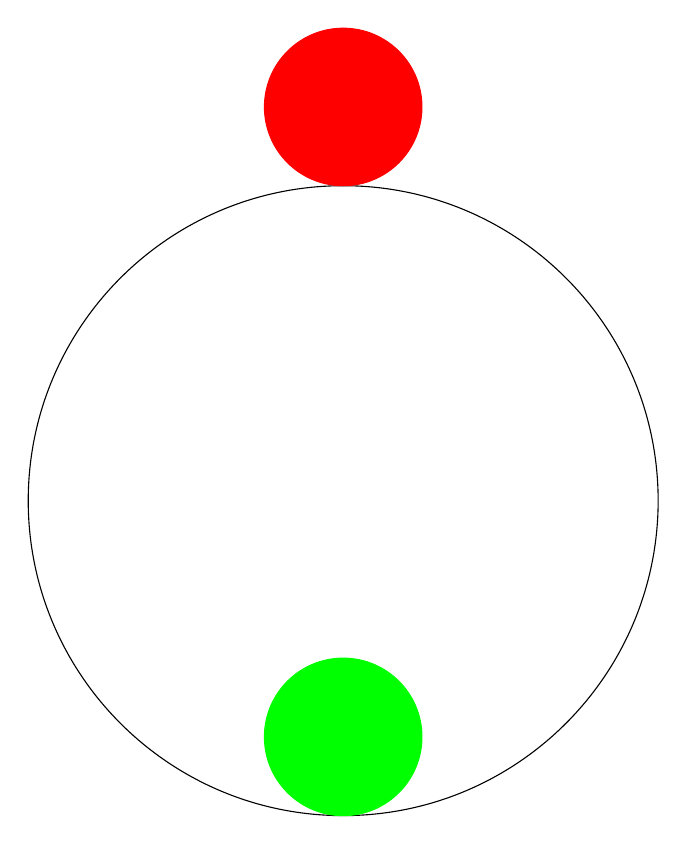
\begin{tikzpicture}
        \draw[] (0,0) circle (4);
        \draw[color=red,fill] (0,5) circle (1);
        \draw[color=green,fill] (0,-3) circle(1);
    \end{tikzpicture}
\end{center}
\begin{itemize}
    \item The red circle is in unstable equilibrium. The green circle is in stable equilibrium.
    \item Something resting on the saddle point of $y=x^3$ will be in semistable equilibrium.
\end{itemize}
\begin{example}
    Find and classify the equilibria of the ODE $y'=3\cos y$
    \begin{center}
        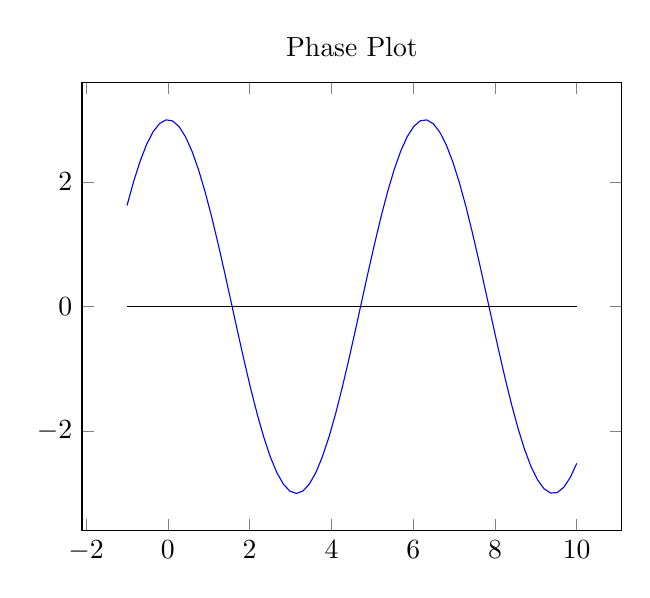
\begin{tikzpicture}
            \begin{axis}[title=Phase Plot]
                \addplot [
            domain=-1:10,
            samples=70,
            color=blue,
            ]
            {3*cos(x*57.2958)};
            \addplot [
                domain=-1:10,
                samples=70,
                color=black,
                ]
                {0};            
            \end{axis}
        \end{tikzpicture}
    \end{center}
\end{example}
\begin{sol}
    To find equilibrium, set $y'=0$.
    \begin{align}
        y'&=3\cos y=0\\
        y&=\frac{\pi}{2}+n\pi,n\in\mathbb Z
    \end{align}
    At the equilibrium at $y=\frac{\pi}{2}$, In the phase diagram, anything below or above it s
\end{sol}


\end{document}